\section{Talkgroup Betrieb} \label{sec:talkgroup}
Ein klassisches und auch schönes Beispiel für den Repeater-transparenten Sprechgruppenbetrieb (Talkgroup) ist das Szenario einer Nachmittagsrunde in einer Sprechgruppe. Zum Beispiel, die Sprechgruppe 2621 \emph{Berlin/Brandenburg} kurz BB. Diese Sprechgruppe ist bei fast allen Repeatern in Berlin und Brandenburg fest Abonniert. D.h., diese Runde kann ohne weiteres Zutun in ganz Berlin und Brandenburg empfangen werden (siehe Abb. \ref{fig:tgex1}. 

\begin{figure}[p]
 \centering
 \begin{subfigure}{\linewidth}
  \centering
  \documentclass{standalone}
\newcommand{\repeater}[3]{%
 \node ({#1}) at ({#2}) {%
  \begin{tikzpicture}%
   \draw [black,thick] (-.25,0) -- (0,0.5) -- (0.25,0) -- (-0.25,0);%
   \draw [black,thick,domain=-45:225] plot ({0.2*cos(\x)}, {0.5+0.2*sin(\x)});%
   \draw [black,thick,domain=-45:225] plot ({0.4*cos(\x)}, {0.5+0.4*sin(\x)});%
   \node (xxx) at (0,-.2) {{#3}};%
  \end{tikzpicture}%
 } %
}

\newcommand{\activerepeater}[3]{%
 \node ({#1}) at ({#2}) {%
  \begin{tikzpicture}%
   \draw [black,thick] (-.25,0) -- (0,0.5) -- (0.25,0) -- (-0.25,0);%
   \draw [red,thick,domain=-45:225] plot ({0.2*cos(\x)}, {0.5+0.2*sin(\x)});%
   \draw [red,thick,domain=-45:225] plot ({0.4*cos(\x)}, {0.5+0.4*sin(\x)});%
   \node (xxx) at (0,-.2) {{#3}};%
  \end{tikzpicture}%
 } %
}


\newcommand{\user}[3]{%
 \node ({#1}) at ({#2}) {%
  \begin{tikzpicture}%
   \draw [black,fill=black] (-.25,0) -- (0,0.5) -- (0.25,0) -- (-0.25,0);%
   \draw [black,fill=black] (0,.5) circle (.2); %
   \node (xxx) [text width=0.6cm, align=center] at (-.35cm,-.4) {{#3}};%
  \end{tikzpicture}%
 } %
}

\newcommand{\activeuser}[3]{%
 \node ({#1}) at ({#2}) {%
  \begin{tikzpicture}%
   \draw [red,fill=red] (-.25,0) -- (0,0.5) -- (0.25,0) -- (-0.25,0);%
   \draw [red,fill=red] (0,.5) circle (.2); %
   \node (xxx) [text width=0.6cm, align=center] at (-.35cm,-.4) {{#3}};%
  \end{tikzpicture}%
 } %
}

\begin{document}
  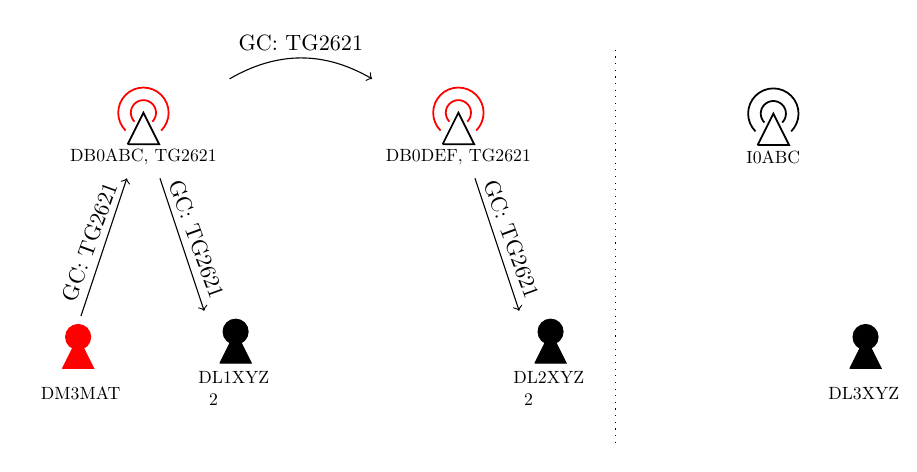
\begin{tikzpicture}[every node/.style={scale=.8}]
   \activeuser{u1}{ 0,0}{DM3MAT};
   \user{u2}{ 2,0}{DL1XYZ 2};	
   \user{u3}{ 6,0}{DL2XYZ 2};	
   \draw[dotted] (7,4) -- (7,-1);
   \user{u4}{10,0}{DL3XYZ};
   \activerepeater{R1}{1,3}{DB0ABC, TG2621};
   \activerepeater{R2}{5,3}{DB0DEF, TG2621};
   \repeater{R3}{9,3}{I0ABC};
   \path[->] (u1) edge node[above,rotate=70]{GC: TG2621} (R1);
   \path[->] (R1) edge node[above,rotate=-70]{GC: TG2621} (u2);
   \path[->] (R2) edge node[above,rotate=-70]{GC: TG2621} (u3);
   \path[->] (R1) edge[bend left] node[above]{GC: TG2621} (R2);
  \end{tikzpicture}
\end{document}

  \caption{Beispiel für eine typische Nachmittagsrunde auf einer Sprechgruppe.} \label{fig:tgex1}
 \end{subfigure}
 \begin{subfigure}{\linewidth}
  \centering
  \documentclass{standalone}
\usepackage{tikz}
\usetikzlibrary{shapes.geometric}
\newcommand{\repeater}[3]{%
 \node ({#1}) at ({#2}) {%
  \begin{tikzpicture}%
   \draw [black,thick] (-.25,0) -- (0,0.5) -- (0.25,0) -- (-0.25,0);%
   \draw [black,thick,domain=-45:225] plot ({0.2*cos(\x)}, {0.5+0.2*sin(\x)});%
   \draw [black,thick,domain=-45:225] plot ({0.4*cos(\x)}, {0.5+0.4*sin(\x)});%
   \node (xxx) at (0,-.2) {{#3}};%
  \end{tikzpicture}%
 } %
}

\newcommand{\activerepeater}[3]{%
 \node ({#1}) at ({#2}) {%
  \begin{tikzpicture}%
   \draw [black,thick] (-.25,0) -- (0,0.5) -- (0.25,0) -- (-0.25,0);%
   \draw [red,thick,domain=-45:225] plot ({0.2*cos(\x)}, {0.5+0.2*sin(\x)});%
   \draw [red,thick,domain=-45:225] plot ({0.4*cos(\x)}, {0.5+0.4*sin(\x)});%
   \node (xxx) at (0,-.2) {{#3}};%
  \end{tikzpicture}%
 } %
}


\newcommand{\user}[3]{%
 \node ({#1}) at ({#2}) {%
  \begin{tikzpicture}%
   \draw [black,fill=black] (-.25,0) -- (0,0.5) -- (0.25,0) -- (-0.25,0);%
   \draw [black,fill=black] (0,.5) circle (.2); %
   \node (xxx) [text width=0.6cm, align=center] at (-.35cm,-.4) {{#3}};%
  \end{tikzpicture}%
 } %
}

\newcommand{\activeuser}[3]{%
 \node ({#1}) at ({#2}) {%
  \begin{tikzpicture}%
   \draw [red,fill=red] (-.25,0) -- (0,0.5) -- (0.25,0) -- (-0.25,0);%
   \draw [red,fill=red] (0,.5) circle (.2); %
   \node (xxx) [text width=0.6cm, align=center] at (-.35cm,-.4) {{#3}};%
  \end{tikzpicture}%
 } %
}

\begin{document}
  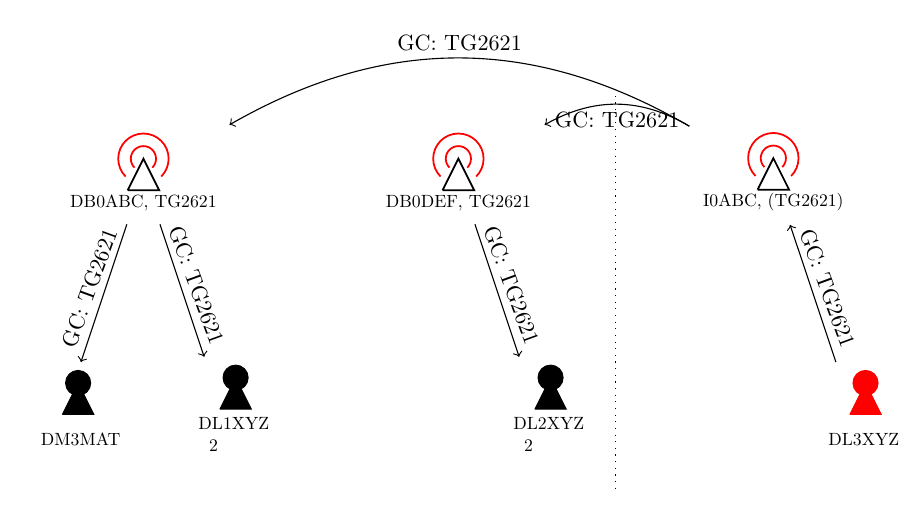
\begin{tikzpicture}[every node/.style={scale=.8}]
   \user{u1}{ 0,0}{DM3MAT};
   \user{u2}{ 2,0}{DL1XYZ 2};	
   \user{u3}{ 6,0}{DL2XYZ 2};	
   \draw[dotted] (7,4) -- (7,-1);
   \activeuser{u4}{10,0}{DL3XYZ};
   \activerepeater{R1}{1,3}{DB0ABC, TG2621};
   \activerepeater{R2}{5,3}{DB0DEF, TG2621};
   \activerepeater{R3}{9,3}{I0ABC, (TG2621)};
   \path[->] (u4) edge node[above,rotate=-70]{GC: TG2621} (R3);
   \path[->] (R1) edge node[above,rotate=70]{GC: TG2621} (u1);
   \path[->] (R1) edge node[above,rotate=-70]{GC: TG2621} (u2);
   \path[->] (R2) edge node[above,rotate=-70]{GC: TG2621} (u3);
   \path[->] (R3) edge[bend right] node[below]{GC: TG2621} (R2);
   \path[->] (R3) edge[bend right] node[above]{GC: TG2621} (R1);
  \end{tikzpicture}
\end{document}

  \caption{Der OM im Ausland abonniert diese Sprechgruppe an dem lokalen Repeater temporär durch einen Gruppenruf zu dieser Sprechgruppe.} \label{fig:tgex2}
 \end{subfigure}
 \begin{subfigure}{\linewidth}
  \centering
  \documentclass{standalone}
\usepackage{tikz}
\usetikzlibrary{shapes.geometric}
\newcommand{\repeater}[3]{%
 \node ({#1}) at ({#2}) {%
  \begin{tikzpicture}%
   \draw [black,thick] (-.25,0) -- (0,0.5) -- (0.25,0) -- (-0.25,0);%
   \draw [black,thick,domain=-45:225] plot ({0.2*cos(\x)}, {0.5+0.2*sin(\x)});%
   \draw [black,thick,domain=-45:225] plot ({0.4*cos(\x)}, {0.5+0.4*sin(\x)});%
   \node (xxx) at (0,-.2) {{#3}};%
  \end{tikzpicture}%
 } %
}

\newcommand{\activerepeater}[3]{%
 \node ({#1}) at ({#2}) {%
  \begin{tikzpicture}%
   \draw [black,thick] (-.25,0) -- (0,0.5) -- (0.25,0) -- (-0.25,0);%
   \draw [red,thick,domain=-45:225] plot ({0.2*cos(\x)}, {0.5+0.2*sin(\x)});%
   \draw [red,thick,domain=-45:225] plot ({0.4*cos(\x)}, {0.5+0.4*sin(\x)});%
   \node (xxx) at (0,-.2) {{#3}};%
  \end{tikzpicture}%
 } %
}


\newcommand{\user}[3]{%
 \node ({#1}) at ({#2}) {%
  \begin{tikzpicture}%
   \draw [black,fill=black] (-.25,0) -- (0,0.5) -- (0.25,0) -- (-0.25,0);%
   \draw [black,fill=black] (0,.5) circle (.2); %
   \node (xxx) [text width=0.6cm, align=center] at (-.35cm,-.4) {{#3}};%
  \end{tikzpicture}%
 } %
}

\newcommand{\activeuser}[3]{%
 \node ({#1}) at ({#2}) {%
  \begin{tikzpicture}%
   \draw [red,fill=red] (-.25,0) -- (0,0.5) -- (0.25,0) -- (-0.25,0);%
   \draw [red,fill=red] (0,.5) circle (.2); %
   \node (xxx) [text width=0.6cm, align=center] at (-.35cm,-.4) {{#3}};%
  \end{tikzpicture}%
 } %
}

\begin{document}
  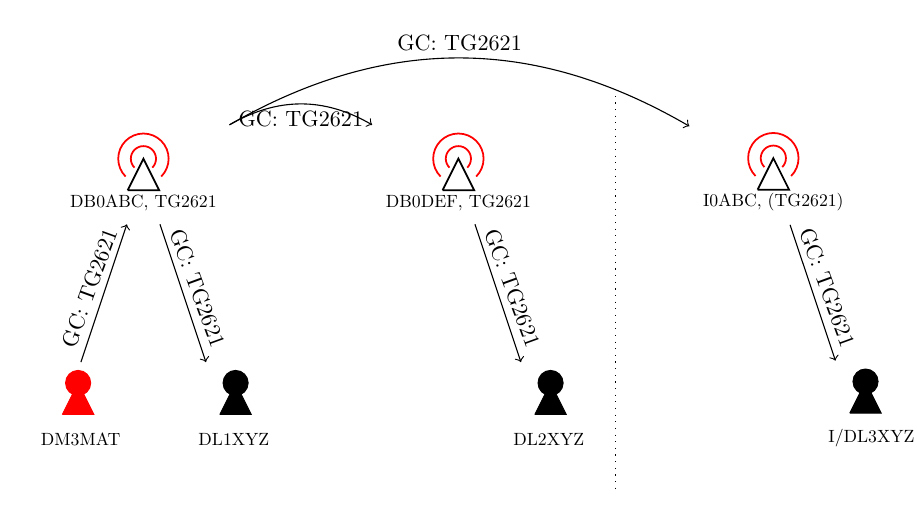
\begin{tikzpicture}[every node/.style={scale=.8}]
   \activeuser{u1}{ 0,0}{DM3MAT};
   \user{u2}{ 2,0}{DL1XYZ};	
   \user{u3}{ 6,0}{DL2XYZ};	
   \draw[dotted] (7,4) -- (7,-1);
   \user{u4}{10,0}{I/DL3XYZ};
   \activerepeater{R1}{1,3}{DB0ABC, TG2621};
   \activerepeater{R2}{5,3}{DB0DEF, TG2621};
   \activerepeater{R3}{9,3}{I0ABC, (TG2621)};
   \path[->] (u1) edge node[above,rotate=70]{GC: TG2621} (R1);
   \path[->] (R1) edge node[above,rotate=-70]{GC: TG2621} (u2);
   \path[->] (R2) edge node[above,rotate=-70]{GC: TG2621} (u3);
   \path[->] (R3) edge node[above,rotate=-70]{GC: TG2621} (u4);
   \path[->] (R1) edge[bend left] node[below]{GC: TG2621} (R2);
   \path[->] (R1) edge[bend left] node[above]{GC: TG2621} (R3);
  \end{tikzpicture}
\end{document}

  \caption{Danach kann auch der OM im Urlaub wie gewohnt an dieser Nachmittagsrunde teilnehmen.} \label{fig:tgex3}
 \end{subfigure}
\end{figure}

Für einen OM im Urlaub, gilt das natürlich nicht. Ein italienischer Repeater wird sicher nicht standardmäßig die Sprechgruppe \emph{Berlin/Brandenburg} abonniert haben. Daher wird dieser OM die Sprechgruppe im Ausland auch nicht hören. Da er aber weiß, wann diese Runde beginnt, kann er vorher per Gruppenruf zu dieser Sprechgruppe von seinem Urlaubsrepeater (I0ABC) aus, diese Sprechgruppe temporär abonnieren (Abb. \ref{fig:tgex2}). 

Nachdem er aber diese Sprechgruppe beim Urlaubsrepeater abonniert hat, kann er wie gewohnt an der Nachmittagsrunde teilnehmen (Abb. \ref{fig:tgex3}). Für die anderen Teilnehmer dieser Runde ist dann nicht einmal ersichtlich, dass der Urlauber nicht über ein Relais in Berlin oder Brandenburg sondern aus dem Ausland and der Runde teilnimmt.

\begin{table}[!h]
 \centering
 \begin{tabular}{|l|c|} \hline
  Name & Sprechgruppe \\ \hline
  Global & 91 \\
  Europa & 92 \\
  Deutschland & 262 \\
  Mecklenburg-Vorpommern \& Sachsen-Anhalt & 2620 \\
  Berlin \& Brandenburg & 2621 \\
  Hamburg \& Schleswig-Holstein & 2622 \\
  Niedersachsen \& Bremen & 2623 \\
  Nordrhein-Westfalen & 2624 \\
  Rheinland-Pfalz \& Saarland & 2625 \\
  Hessen & 2626 \\
  Baden-Württemberg & 2627 \\
  Bayern & 2628 \\
  Sachsen \& Thüringen & 2629 \\ \hline
 \end{tabular}
 \caption{} \label{tab:talkgroups}
\end{table}

\subsection{Cluster}
Im Gegensatz zur dediziert Regionalen Gruppe TG8, sind gewöhnliche Sprechgruppen von überall aus dem DMR Netz erreichbar. D.h., ein OM der sich gerade im Urlaub befindet und an dieser Runde in dieser Sprechgruppe teilnehmen möchte, kann dies wie oben beschrieben tun. Würde diese Nachmittagsrunde aber auf der regionalen Sprechgruppe TG8 stattfinden, könnte der OM im Urlaub nicht daran teilnehmen. Würde er an seinem Urlaubsrepeater einen Gruppenruf zur Sprechgruppe TG8 starten, würde er nur Funkamateure in seiner Urlaubsregion erreichen aber nicht den regionalen Verbund von Repeatern zu Hause.

Aus diesem Grund werden häufig regionale Verbünde von Repeatern mit sogenannten \emph{Clustern} verbunden. Diese \adef{Cluster} stellen dann eine weitere Sprechgruppennummer für den regionalen Verbund zur Verfügung, sodass die Sprechgruppe TG8 einer bestimmten Region auch von außen erreichbar ist. Eine Liste der Regionalcluster und der dazugehörigen Sprechgruppennummer kann unter \url{http://bm262.de/cluster/} abgerufen werden.
